\chapter{Beta Minimum Features}
\labelChapter{betamin}

\begin{introduction}
  Beta Minimum Features desribes briefly the minimum feature-set for the \textbf{beta} version
  of Frienso.  We have decided to pare down the features with the objective of getting a 
  stable version and can handle 20-100 users and does not easily crash. Below is a list of
  the features needing work and a milestone with attached dates that we \textbf{must} try hard
  to meet on time. 
\end{introduction}
\begin{figure*}[t]
\centering

\subfloat{%
  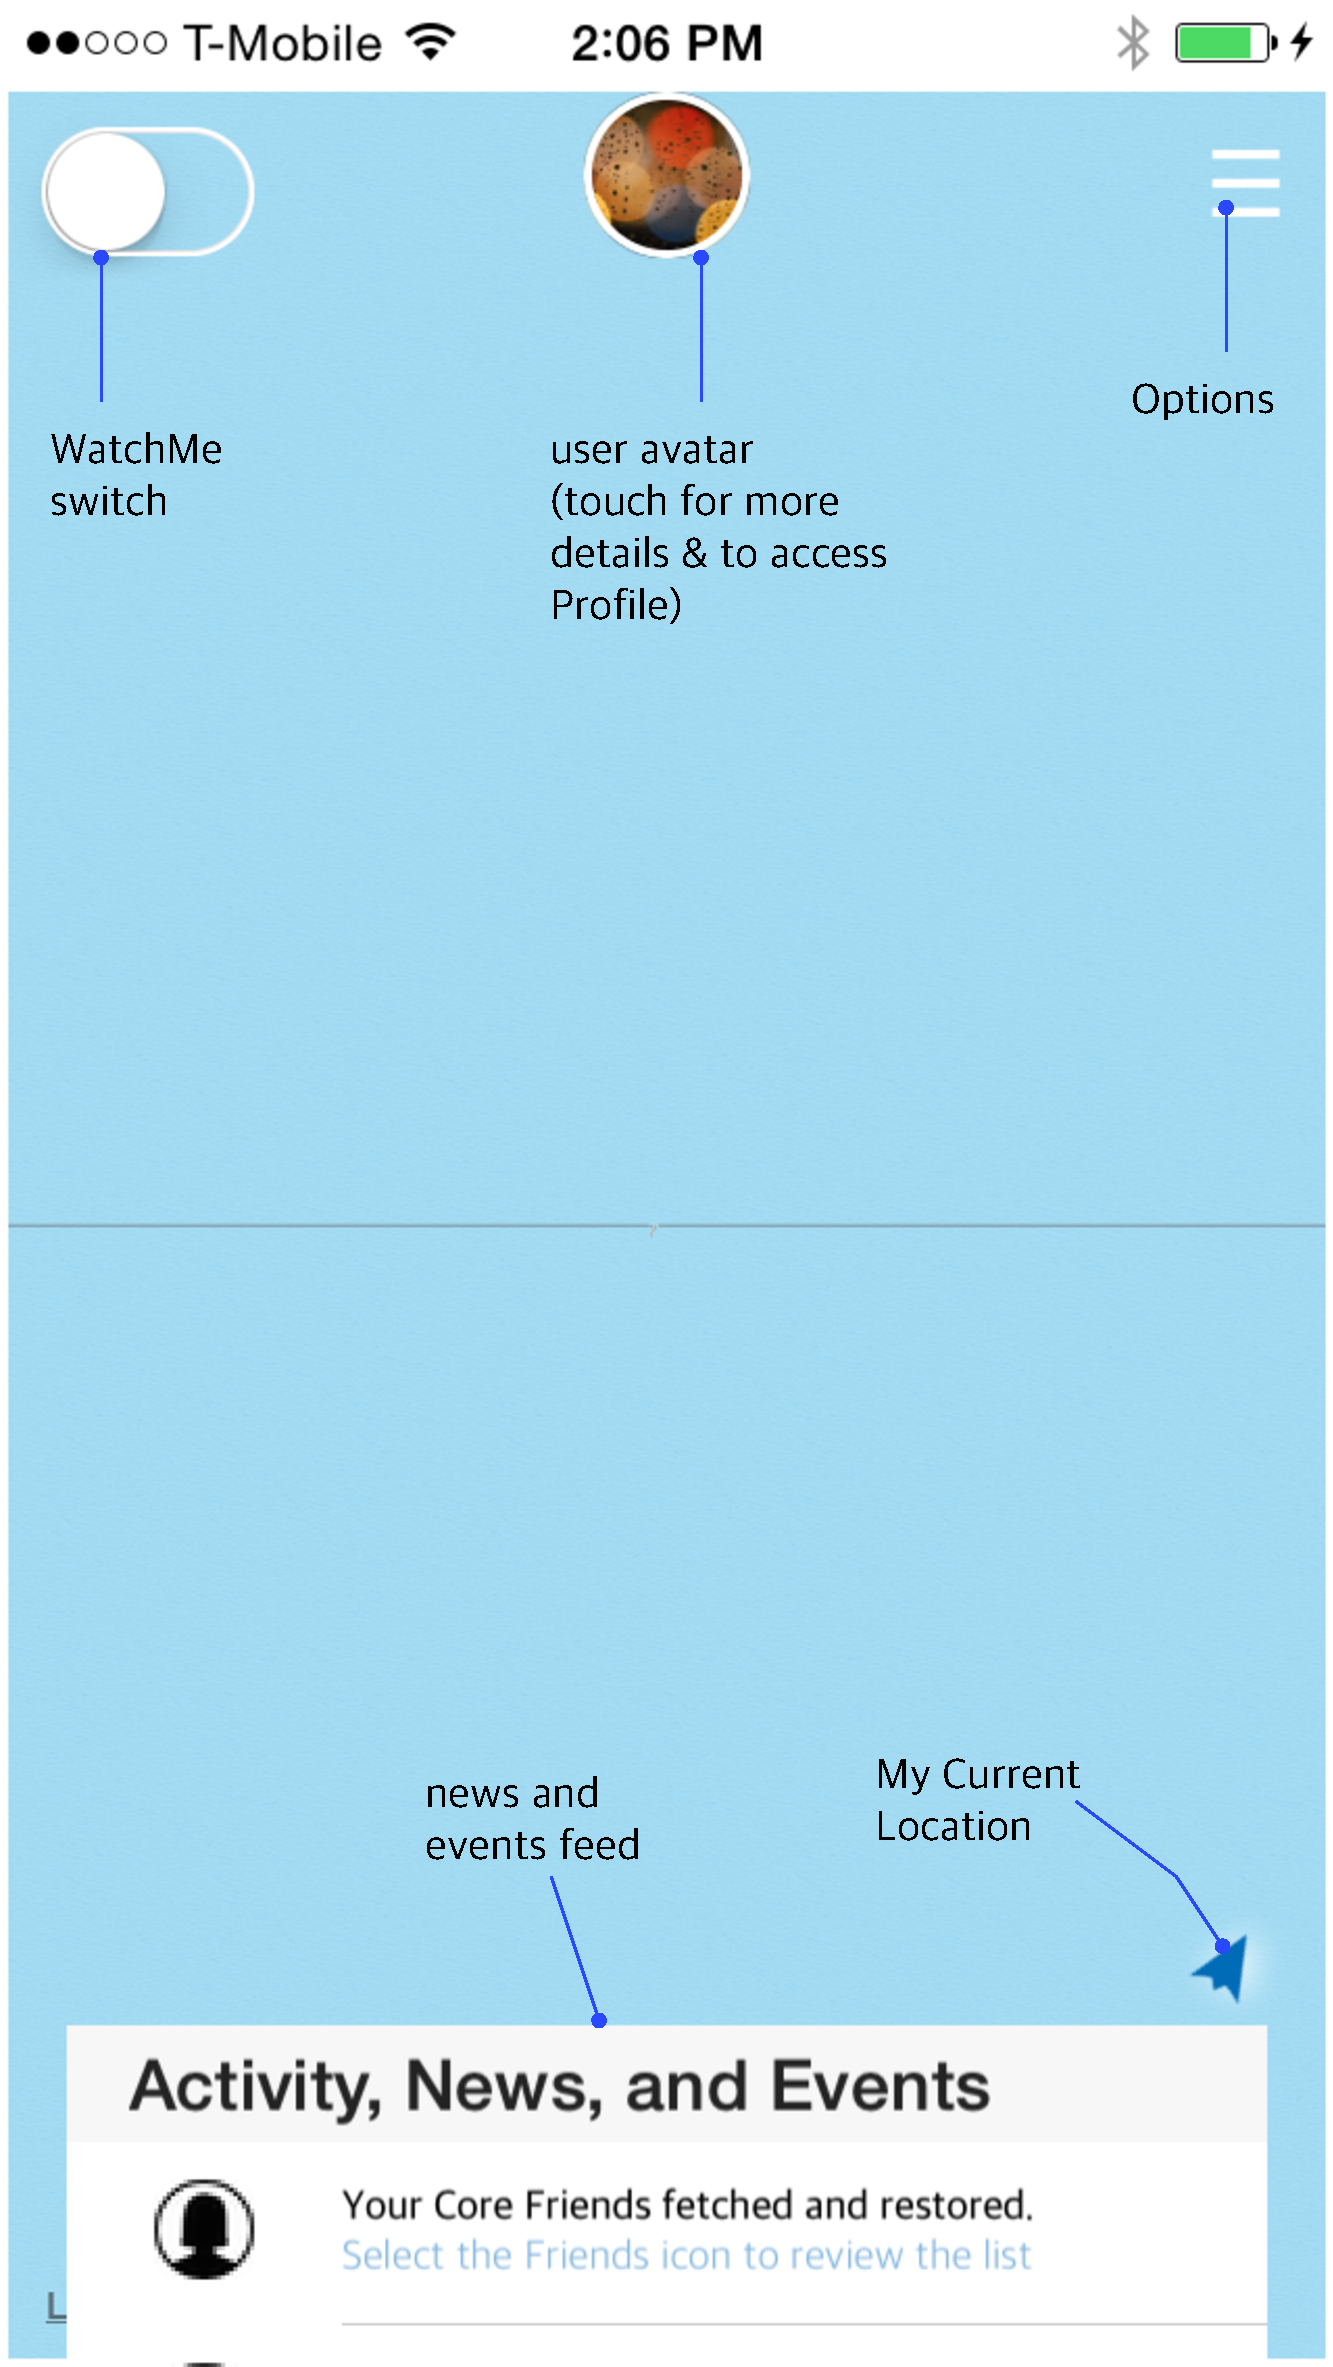
\includegraphics[width=3cm]{images/ScrnSht_mainview}%
    \label{fig:evaluation:revenue}%
}\qquad
\subfloat{%
  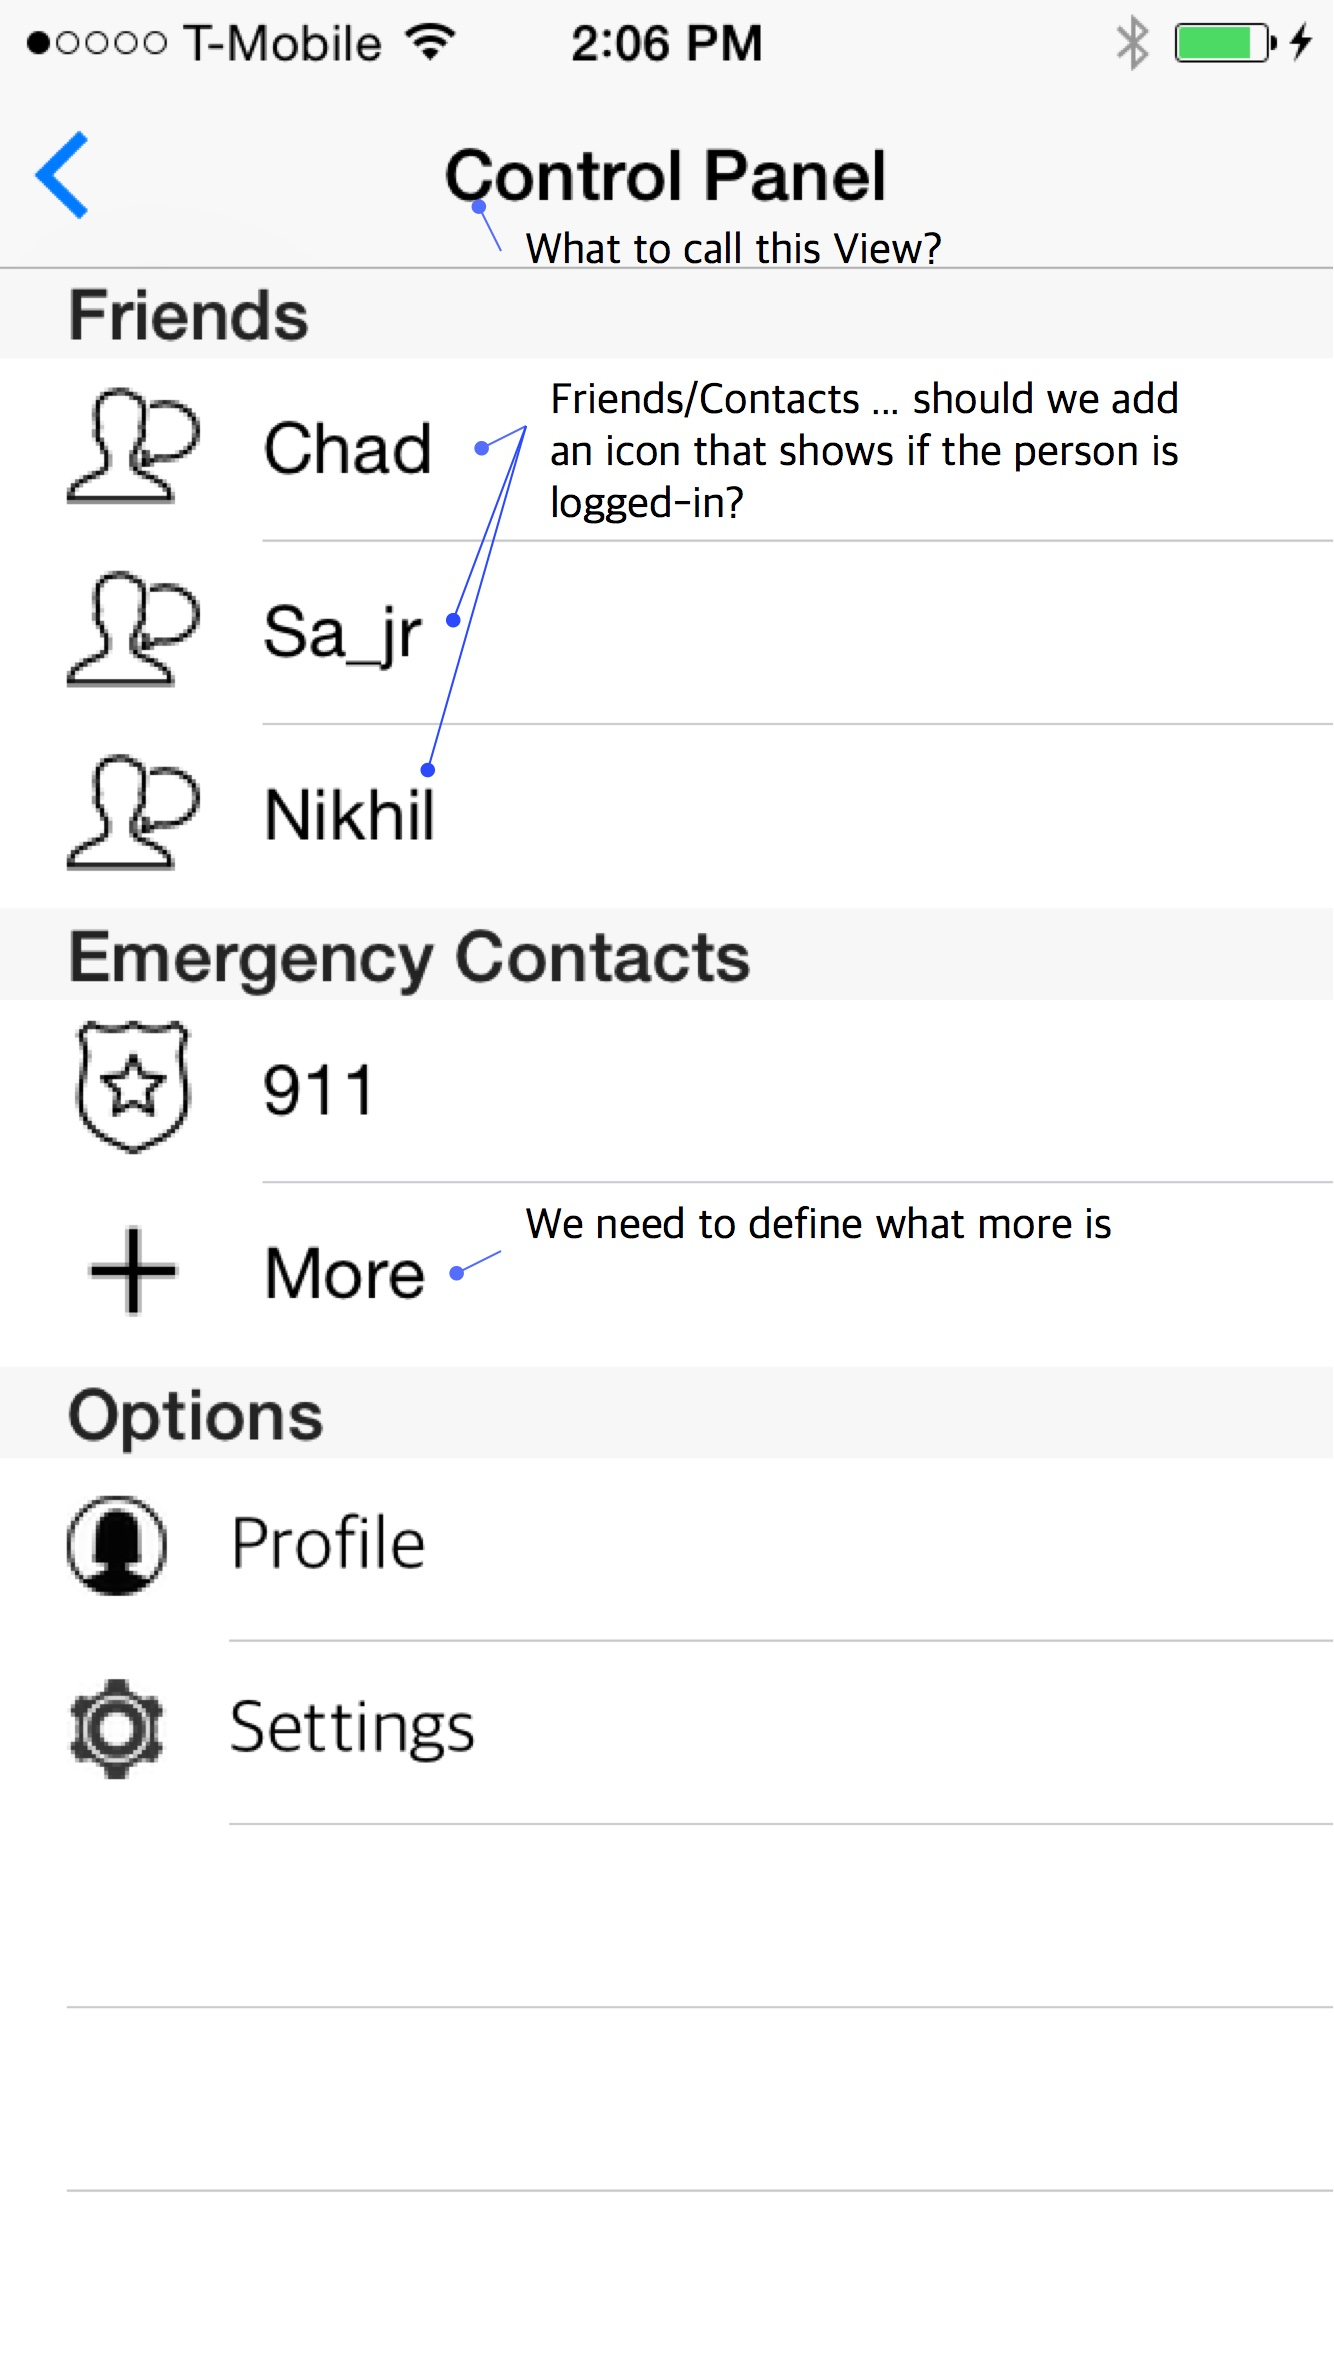
\includegraphics[width=3cm]{images/ScrnSht_optionsview}%
  \label{fig:evaluation:avgPrice}%
}

\caption{Frienso Views: HomeView and the OptionsView}
\end{figure*}

\section{21Dec14 Updates to the MVP}

\begin{enumerate}
\item \textbf{WatchMe:}  We minimize the features, we removed HelpMe for now and make sure WatchMe works by maintaining location info for the duration of WatchMe.
\item \textbf{Friends:} Simplify adding friends to core circle. Eliminate the need for accepting friend requests for now. If the user is in your Contacts, just add the user to the core circle.  On the backend, we maintain only the phone, until that user registers a Frienso account.
\item \textbf{Map location tracking:} Add history/path tracking for the duration of the Watch.
\item \textbf{Design challenges}: What is the best way to query the UserEvents class (data-store for watchMe events)
so that we don't pull 10s, 100s, 1000s of active events when we begin to scale up? We need a design improvement
to post an event (say watchMe) and that user's event is stored in cloud with properties that limits a query to only those that the user's micro-network. /NY?/

\end{enumerate}

\subsection{Issues due to iOS, and Mac OS updates}
Selecting contacts has changed in iOS 8.  There are now new requirements for building the apps to be both 32 and 64 bit compatible. We need to look into that. There are tons of deprecations for iOS 8.1\\

We need to change the crash reporting (use Parse's new offering). \\

Current iOS version (repository): branch \emph{ frienso\_beta\_experimental} \\

\subsection{Map Location Tracking}
\noindent\textbf{Proposal for review:} (sal) I propose that after a user enables watchMe, the user's device
updates location every so many seconds using the normal way of location updating. Then on the user's side, those
watching will fetch (get) the corefriend's location with the watchMe event. For that user we maintain 
a route array of geopoints.  The aim is to simplify and minimize our backend storage and its complexity,
so that we may avoid/minimize app errors.

\section{21Dec14 Action Items}
\subsection{iOS version}
See table~\ref{tab:ios}.
\begin{table}[!htb]
\renewcommand\arraystretch{1.3}
%\renewcommand\tabcolsep{0pt}
  \caption{iOS Version: action items}\label{tab:ios}
  \begin{tabular*}{\textwidth}{@{\extracolsep{\fill}}l|l}
  \textbf{Task} & \textbf{Owner} \\\toprule
  Map/route tracking & Sal \\
  Contacts selection (adding friends to core friends) & Sal \\
  Compatibility issues with new iOS and new dev tools & Nikhil \\
  Make new minimal iOS home-view work & Nikhil \\
  \midrule
  \textbf{Milestone:} Release new version with changes above& N/S by 01Jan15 \\
		\end{tabular*}
		\end{table}
\subsection{Android Version}
See table~\ref{tab:andr}.
\begin{table}[!htb]
\renewcommand\arraystretch{1.3}
%\renewcommand\tabcolsep{0pt}
  \caption{Android Version: action items}\label{tab:andr}
  \begin{tabular*}{\linewidth}{@{\extracolsep{\fill}}l|l}
  \textbf{Task} & \textbf{Owner} \\\toprule
  ** task description ** & Udayan \\
  ** unit testing ** & U/N/S \\
  \midrule
  \textbf{Android Milestone } Release new version & Udayan by (date)\\
        \end{tabular*}
        \end{table}

\color{gray}
\section{24Jun14 Status of the MVP} 

Dev Team has met with Mudit and adopted some of his design suggestions.  
\begin{itemize}
\item In-app chatting is postponed, but we really need this feature working b/c otherwise it is a boring app
\item Push notifications are now working on the development versions (we haven't made a distribution executable to share with the rest of the team but will be done later this week).
\item CoreCircle creation and editing is currently giving us some issues b/c it prevents the user from creating or editing the mCircle and interacting with it immediately.  Nikhil and Sal have discussed the idea of allowing users to use, view, and interact with the circle until an individual rejects to be added to one's coreCircle.  This can be expanded separately.
\item Event handling: watchMe events are working and tested under diff. conditions (design doc will expand on the various scenarios); HelpMeNow events Nikhil to finalize in the next couple of days. 
\item Pre-populated School emergency contacts now occur when the app is first installed, so it's working.  They are cached locally so user will always know and have these contacts available.
\item The HomeView now has:
\subitem{$\cdot$} WatchMe switch that works by sharing location information until the user turns it off.
\subitem    A map that tracks: watchMe events and HelpMeNow events (currently not working/implemented)
\subitem    Buttons to refresh PendingRequests, buttons to switch between fullscreen Map and standard size
\subitem    Pending requests slider+drawer that holds WatchMe and CoreFriend requests from Frienso users
\subitem    An events listView that can be toggled between minimized and fullscreen by swiping
\subitem    A toolbar (bottom of the screen) with 3 buttons:  Your List of Friends, HelpMeNow trigger, and a Settings view
\subitem    In Settings View we have limited the options to: Profile, Resources, and we think that Settings and About will merge into About Frienso or something like that.

\item Action Items from the Dev Team: 

\subitem    Get HelpMeNow events working 
\subitem    Settle on the look and feel of the events list view at the bottom of the Home View
\subitem    Finish/Improve the Welcome View

\item Action Items for the whole Founders team:

\subitem    Edit and optimize key wording (e.g. slogans and what we name those in our core circle of friends (iCore Friends  as in inner core friends vs. those we watch they have added us to their core circle, so oCore Friends, as in outer Core Friends?).   We need a unified slogan for the app and our literature:  "FRIENSO, be safe with friendso" vs. "FRIENSO, Your $\mu$Social Safety Network for College Campus"
\end{itemize}


%\begin{table}[!Ht] 
%\begin{minipage}{0.49\textwidth}
%\centering\small\renewcommand*{\arraystretch}{1.5} 
%\caption[]{Partial Database Table Structure}\label{tbl:dbstruc} 
%\begin{tabularx}{1\textwidth}{p{.2\textwidth}p{.25\textwidth} p{.475\textwidth}} % - 2\tabcolsep}
%\begin{tabular}{1\textwidth}{X|X|X|X|X|X|X}
%\begin{tabular}{c|c|c|c|c|c|c}
%\begin{tabular*}{\columnwidth}{@{\extracolsep{\stretch{1}}}*{7}{c}@{}}
%\begin{tabular*}{\columnwidth}{@{\extracolsep{\stretch{1}}}*{7}{c}@{}}
%-----------
%\begin{tabularx}{1\textwidth}{X|X}
%\hline
%\textbf{Instructors:} & Sal and Nikhil \\
%\textbf{Office Hours:} &  \\
%\textbf{Pre-requisites:} & \\
%\textbf{Suggested Books} &   \\
%\textbf{Course Outline} & \\
%\textbf{Instructors:} & Sal and Nikhil \\
%\midrule
%\textbf{Dates:} & \textbf{Description} \\
%\toprule 
% -----------

%\end{tabular*} \end{minipage} 
%\end{table}
